\section{Analysis}

\begin{definition}[Entropic Growth]
  The \emph{Entropic Growth} property of
  a \poem execution,
  parametrized by the growth interval $s \in \mathbb{N}$
  and the growth velocity $\tau \in \mathbb{R}^+$,
  states that for
  all honest parties $P$ and all rounds $r_1 + s \leq r_2$,
  the chains $C_1, C_2$ of $P$ at rounds $r_1, r_2$ respectively
  satisfy $\work(C_2[{|C_1|}{:}]) \geq s \tau \lg T$.
\end{definition}

\begin{definition}[Entropic Quality]
  The \emph{Entropic Quality} property of
  a \poem execution, parametrized by the \emph{quality chunk parameter} $\ell \in \mathbb{N}$
  and \emph{quality concentration parameter} $\mu \in \mathbb{R}^+$
  (with $\ell \mu \geq 1$)
  states that for
  all honest parties $P$ and all rounds $r$,
  the chain $C$ of $P$ at round $r$
  has the property that
  for every $0 \leq \alpha < \work(C) - \ell \lg T$,
  there is at least one honestly generated block in the chain
  $[{\alpha}{:}{\alpha + \ell \lg T}] \lhd C$.
\end{definition}

\begin{definition}[Entropic Common Prefix]
  The \emph{Entropic Common Prefix} property of
  a \poem execution, parametrized by the \emph{common prefix parameter} $k \in \mathbb{N}$
  states that for
  all honest parties $P_1, P_2$
  and all rounds $r_1 \leq r_2$,
  the chains $C_1, C_2$ of $P_1, P_2$ at rounds $r_1, r_2$ respectively
  satisfy $[{:}{-k \lg T}] \lhd C_1 \preceq C_2$.
\end{definition}

\begin{conjecture}[Entropic Growth]
  Typical executions of \poem satisfy the Entropic Growth property
  with $s = \lambda$ and $\tau = (1 - \epsilon)f$.
\end{conjecture}

\begin{conjecture}[Entropic Quality]
  Typical executions of \poem satisfy the Entropic Quality property
  with $\ell = 2 \lambda f$ and
  $\mu = 1 - (1 + \frac{\delta}{2})\frac{t}{n - t} - \frac{\epsilon}{1 - \epsilon}$.
\end{conjecture}

\begin{conjecture}[Entropic Common Prefix]
  Typical executions of \poem satisfy the Entropic Common Prefix property
  with $k = 2 \lambda f$.
\end{conjecture}

Consider an execution of the \poem protocol.

We define a discrete and uniformly random variable $X_{r, i}$ as follows.
\atnote{$X_{r, i}$ is not uniformly random}
If at round $r$, honest party $P_i$ finds PoW block $B$, then $X_{r, i} = \work(B)$.
If no PoW is found, $X_{r, i} = 0$. We define $X_{r}$ as the maximum PoW intrinsic work
generated by an honest party during round $r$. Hence, $X_{r} = \max_{i = 1}^{n - t}{X_{r,i}}$.

Next, we define a discrete random variable $Z_{r, j, k}$ as follows.
If at round $r$, the $k$-th query of adversarial party $P_j$ is a PoW block $B$, then
$Z_{r, j, k} = \work(B)$. If no PoW is found, $Z_{r, j, k} = 0$. We define $Z_{r}$ as
the sum of all PoW intrinsic work generated by all adversarial party queries
during round $r$. Hence, $Z_{r} = \sum_{j = 1}^{t}{ \sum_{k = 1}^{q}{ Z_{r, j, k} } }$.
\atnote{Maybe call adversarial parties $P_j^{\mathcal{A}}$}

\begin{conjecture}[\poem is Safe]
  Typical executions of \poem are safe.
\end{conjecture}

\begin{conjecture}[\poem is Live]
  Typical executions of \poem are live.
\end{conjecture}

\begin{corollary}[\poem is Secure]
  Typical executions of \poem are secure.
\end{corollary}
\begin{proof}
  Security follows from safety and liveness.
  \Qed
\end{proof}

\begin{figure}[h]
    \centering
    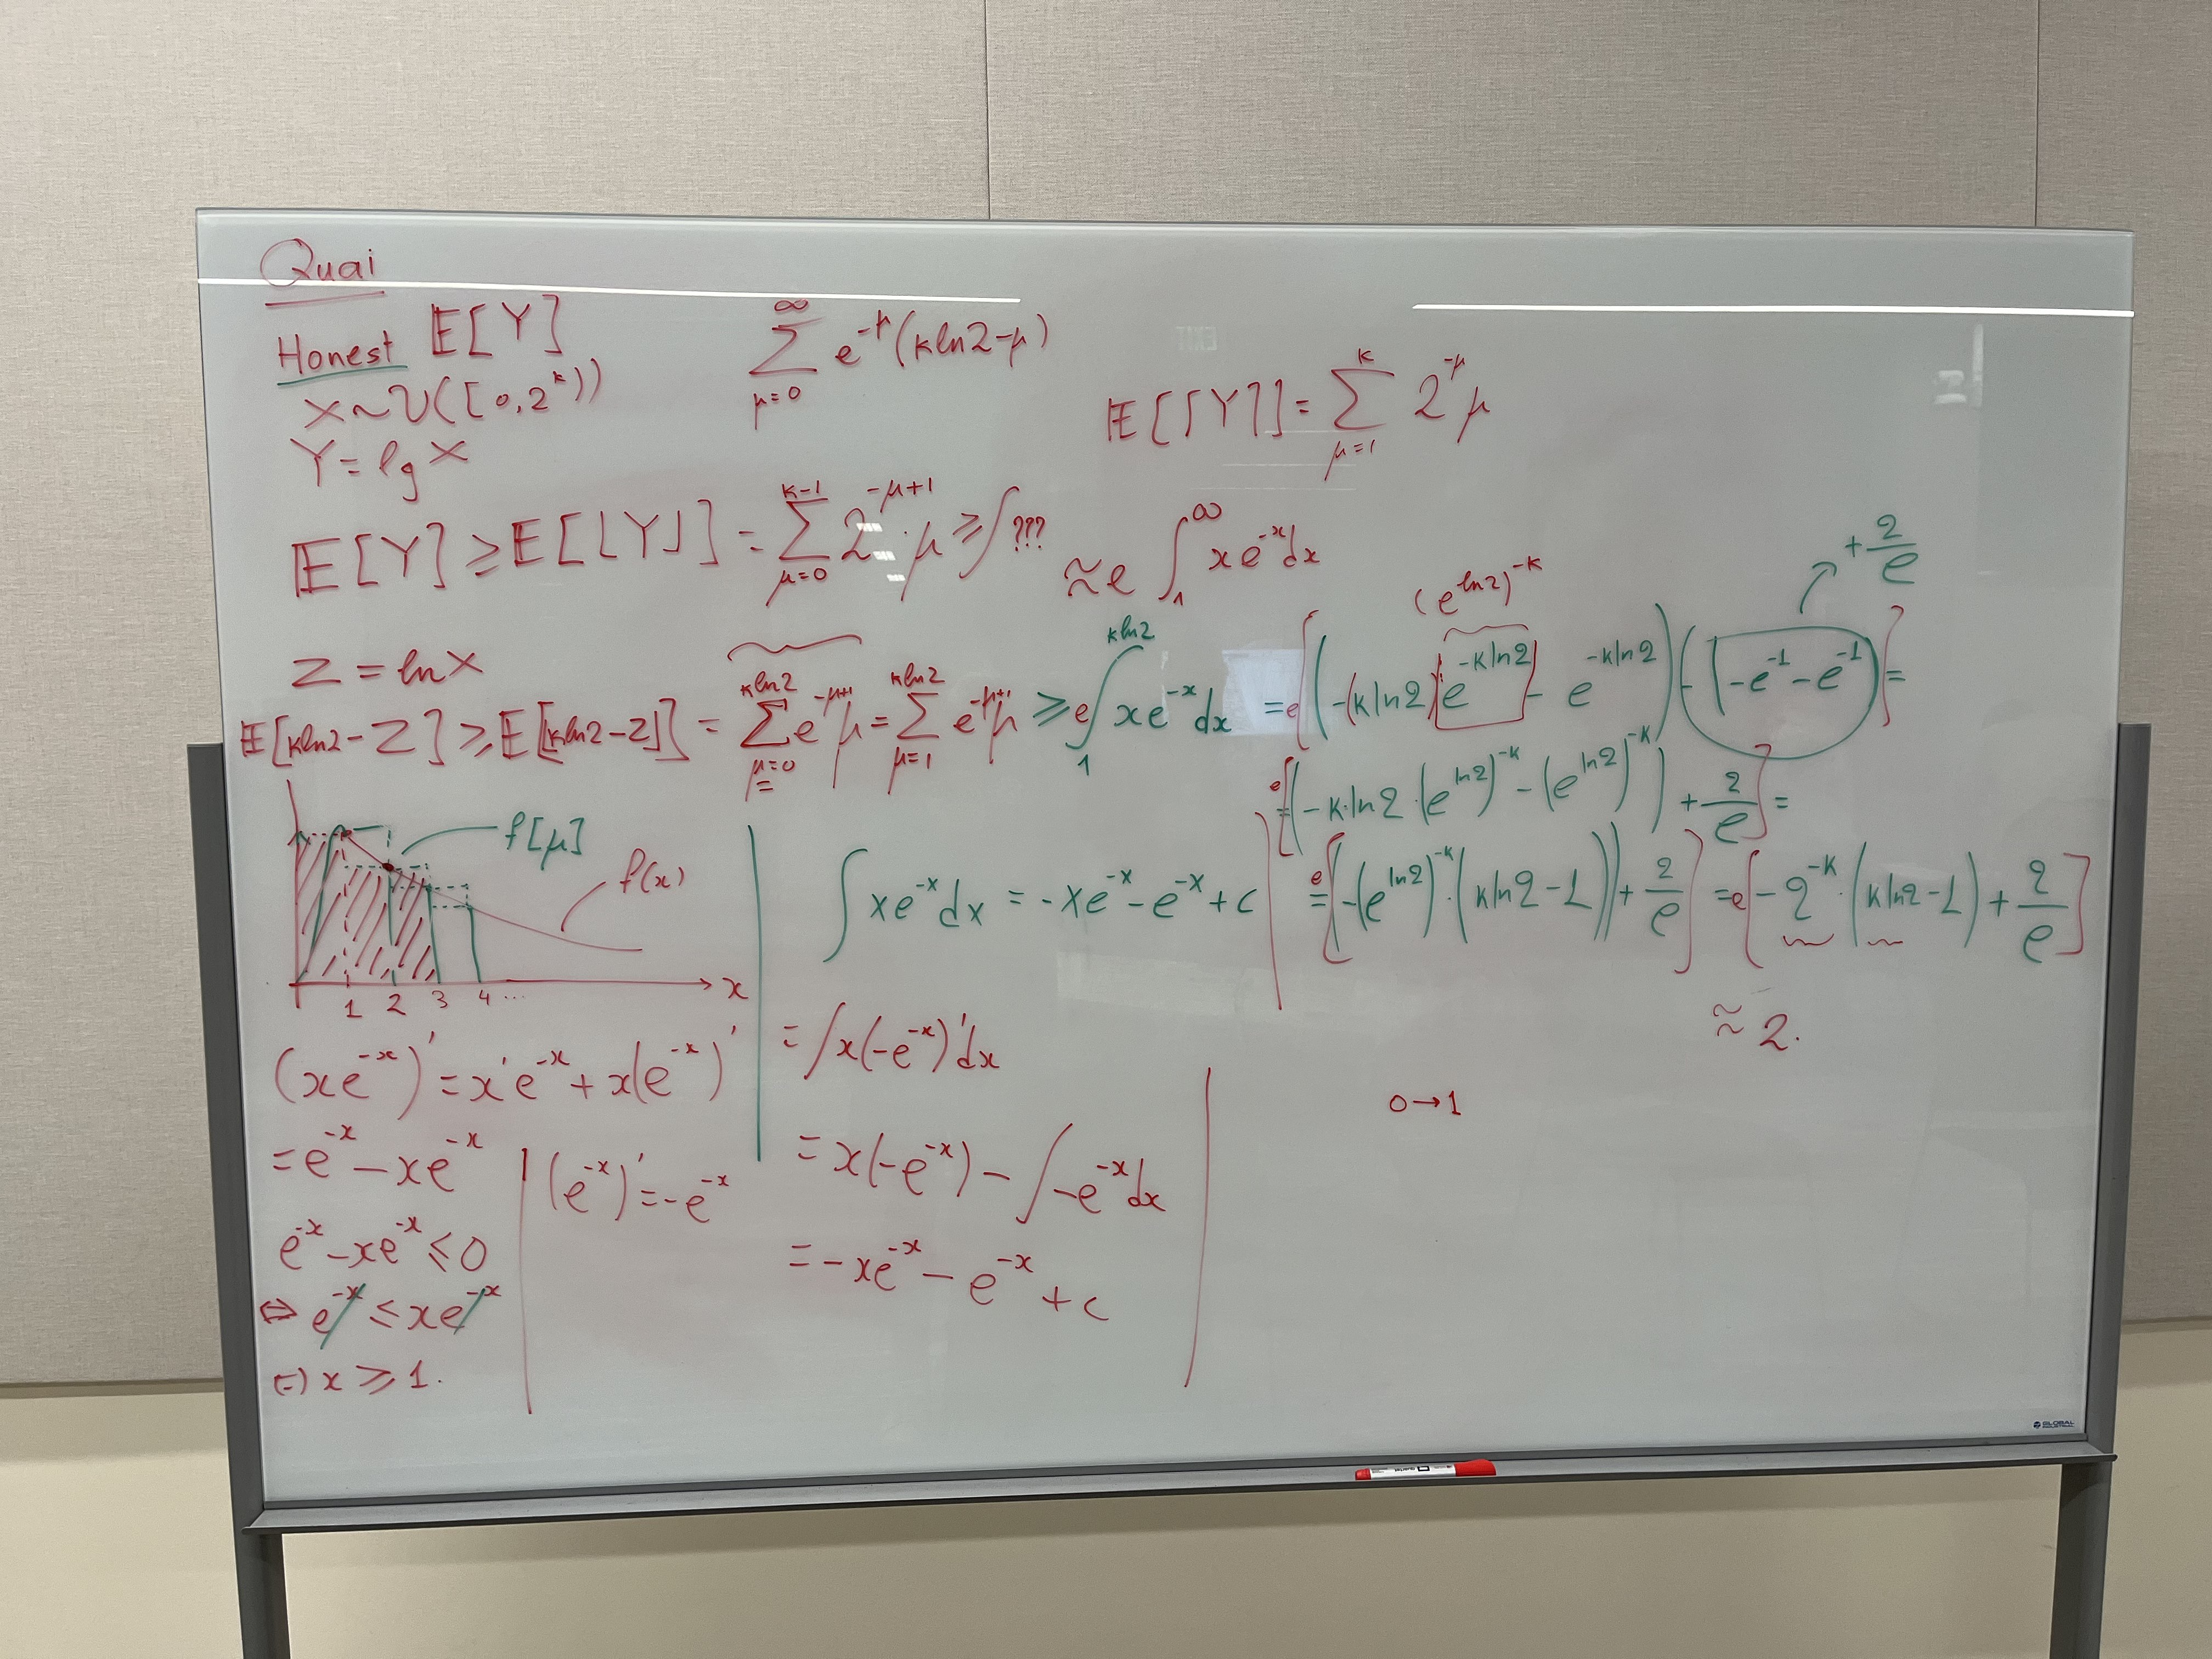
\includegraphics[width=1\textwidth]{figures/bounds-1.jpeg}
\end{figure}

\begin{figure}[h]
    \centering
    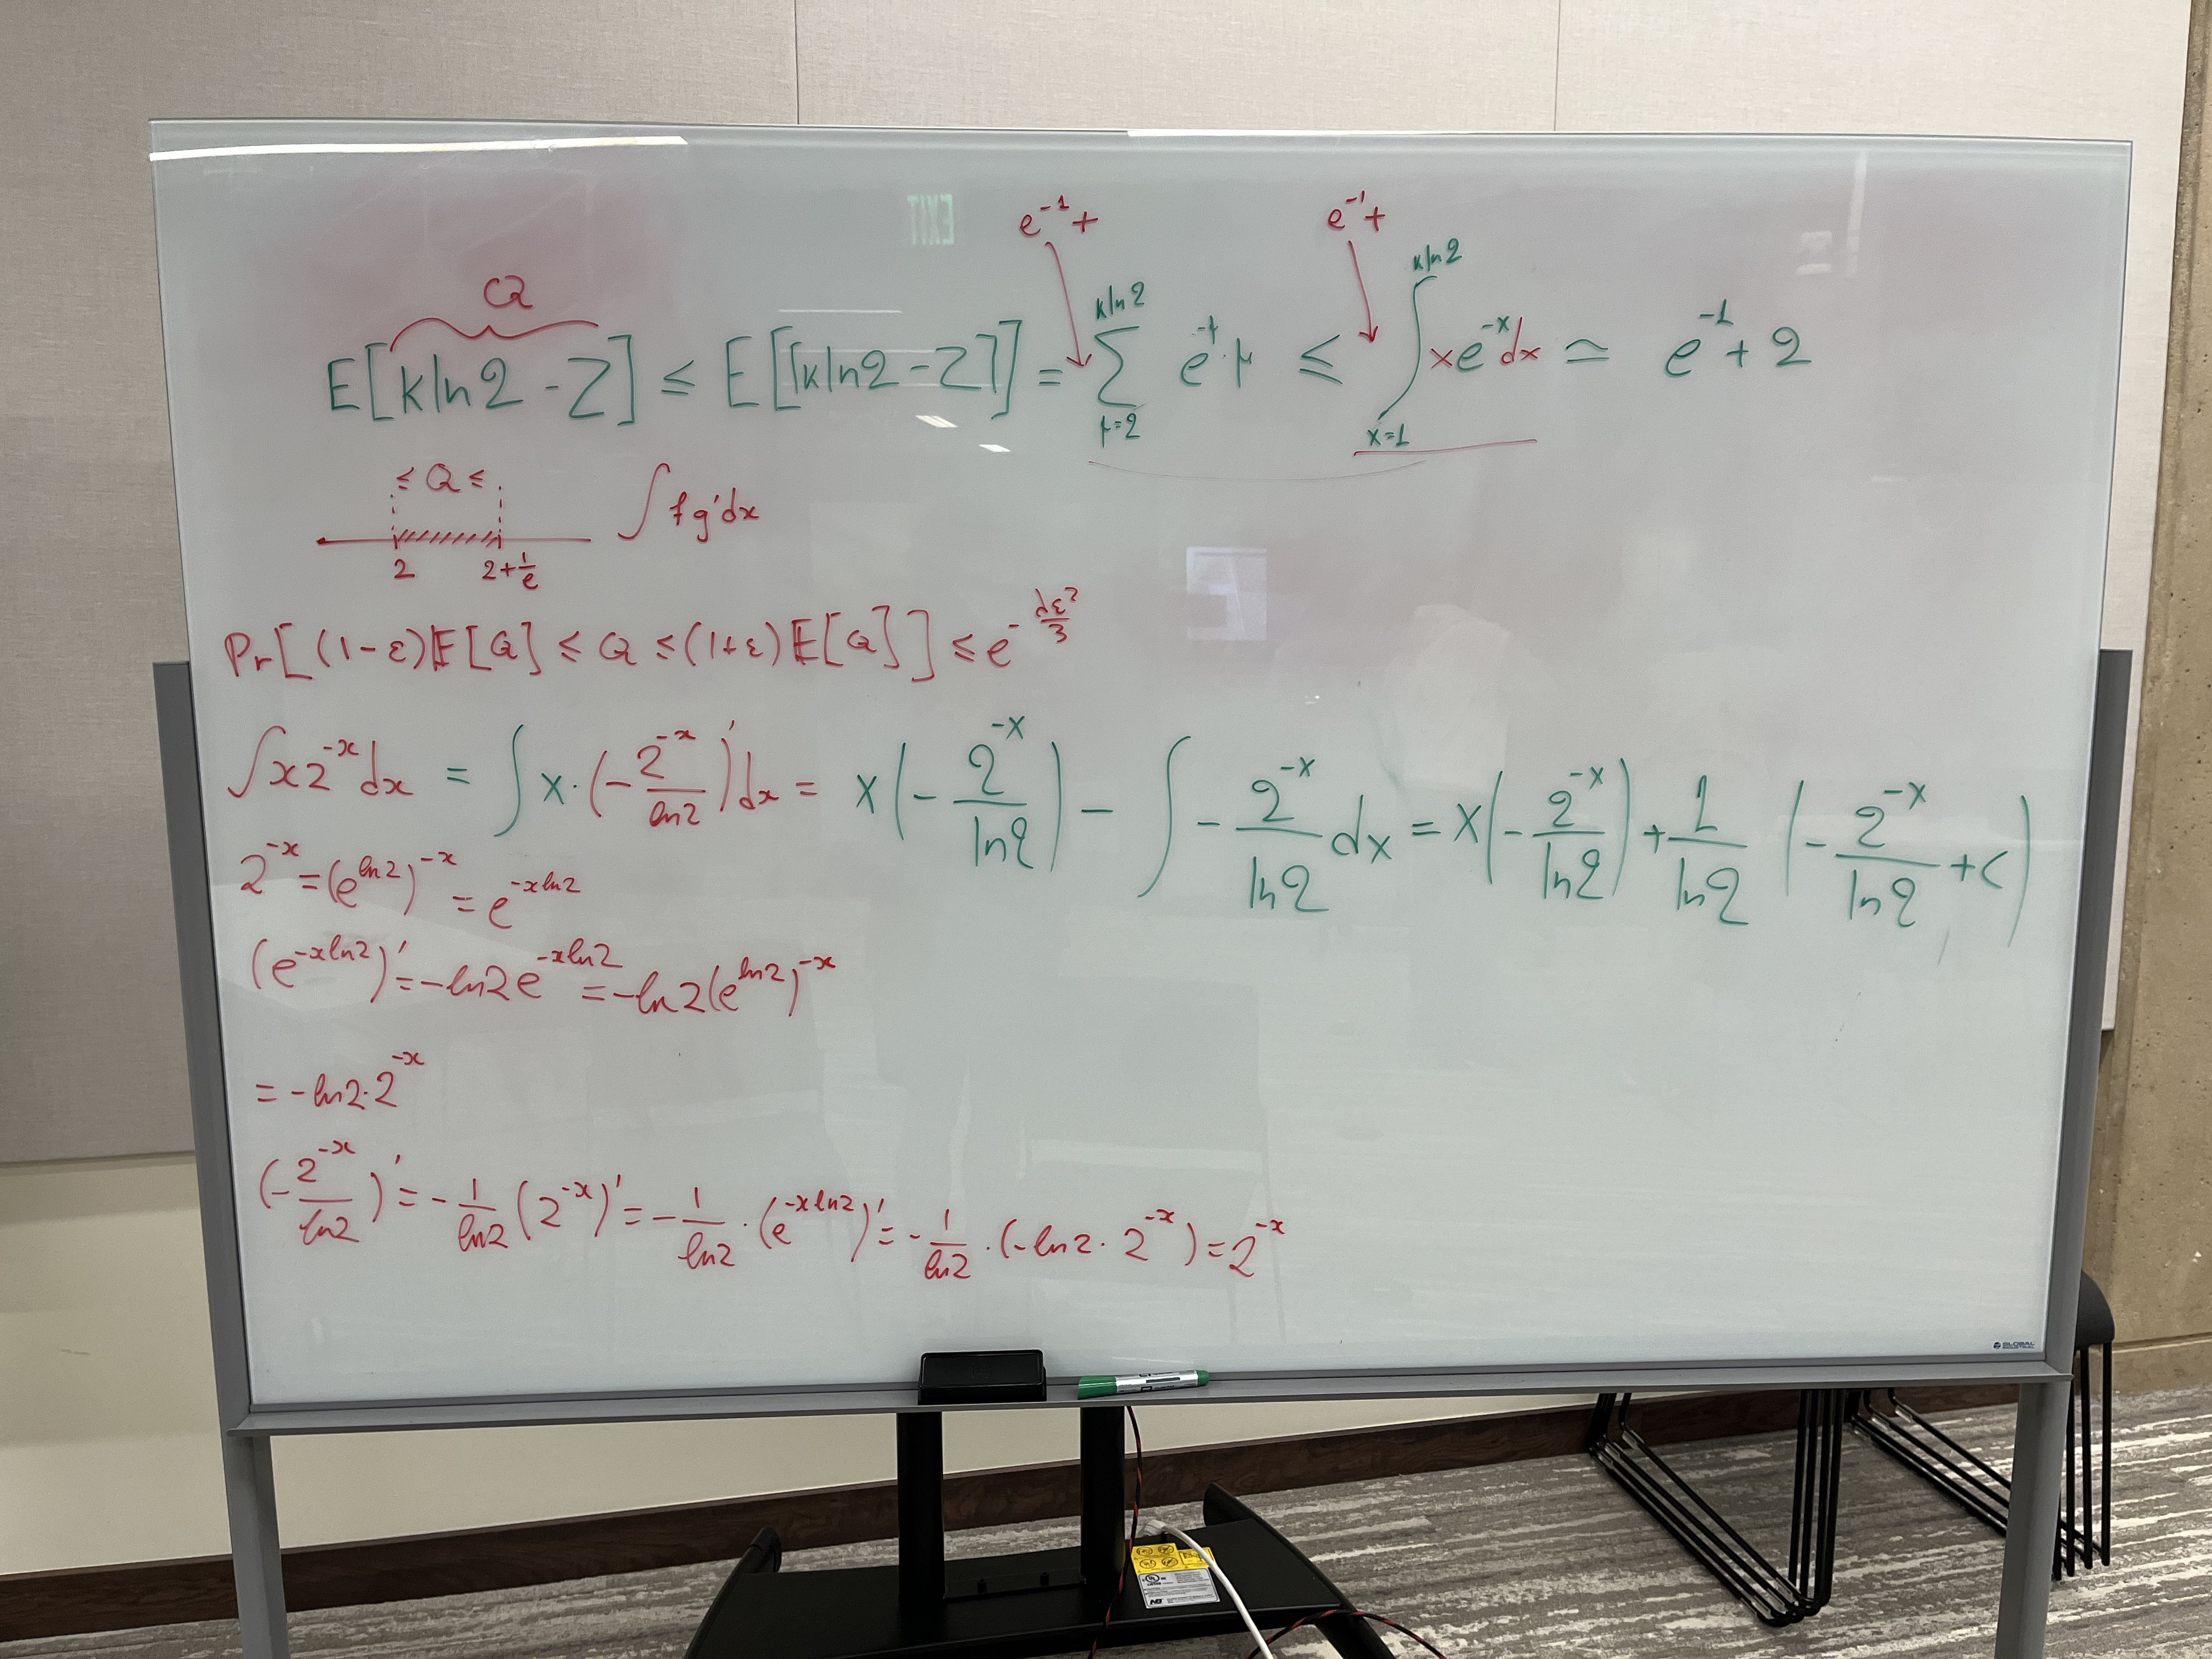
\includegraphics[width=1\textwidth]{figures/bounds-2.jpeg}
\end{figure}
